%-------------------------------------------------------------------------------
\section{Findings}
%-------------------------------------------------------------------------------

Due to the time and resources available for our experiment, our efforts were limited 
to four targets, \texttt{exiv2}, \texttt{infotocap}, \texttt{mp3gain}, and 
\texttt{tcpdump}\textbf{(RQ2)}. Each of these were included in Fu et al.\cite{fu_autofz_2023} 
and are part of

Figure \ref{fig:exiv2_compare_orig_arm64} displays bitmap density covered by the individual algorithms in our ARM64 implementation, 
as compared to a similar plot from Fu et al.\cite{fu_autofz_2023}. While our recreation of autofz achieved lower bitmap coverage than 
the version published by Fu et al., our individual fuzzers also achieved lower bitmap coverage. As a result, our replica still 
outperformed all other individual fuzzers tested in our environment. This is consistant
with Fu et al. findings and further proves that \texttt{autofz} is seperior to individual fuzzers.

\begin{figure}
    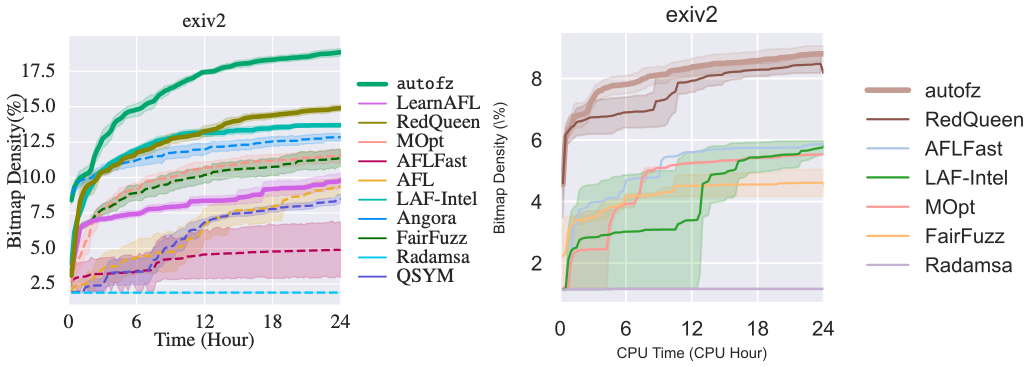
\includegraphics[width=0.52\textwidth]{figs/exiv2_compare_orig_arm64.png}
    \centering
    \caption{A comparison of bitmap density covered in the original\cite{fu_autofz_2023} and our 
    coverage during initial fuzzing of exiv2}
    \label{fig:exiv2_compare_orig_arm64}
\end{figure}

Testing indicates that the ARM64 compatible autofz performs similarly to the unmodified AMD64 \texttt{autofz}. 
Bitmap density coverage of \texttt{autofz} is plottted alogside our ARM64 compatible \texttt{autofz} in figure 
\ref{fig:tcpdump_compare_orig_arm64}. After 24 hours, both implementations achieved similar bitmap coverage.
\texttt{Autofz}'s bitmap coverage grew linearly while ARM64 \texttt{autofz} followed a logarithmic trend. Consequently, 
the orignal \texttt{autofz} took longer to achieve the same bitmap coverage. 

\begin{figure}
    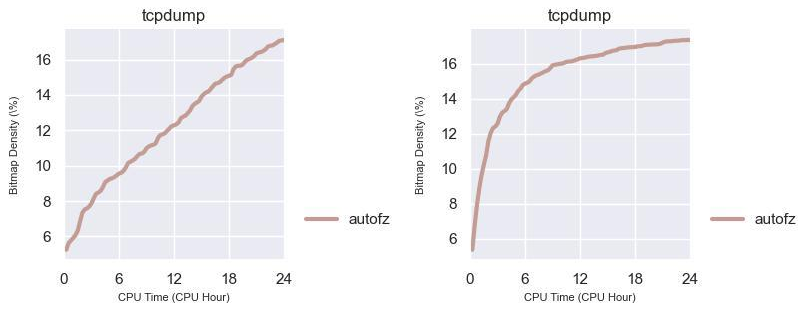
\includegraphics[width=0.52\textwidth]{figs/tcpdump_compare_orig_arm64.png}
    \centering
    \caption{A comparison of bitmap density covered in AMD64 \texttt{autofz} and our ARM64 implementation
    coverage during fuzzing of tcpdump}
    \label{fig:tcpdump_compare_orig_arm64}
\end{figure}

Bug coverage of our ARM64 fuzzing campaign against tcpdump is plotted in figure \ref{figs:tcp_compare_orig_arm64_ub.png}, 
shown as a comparison are results from Fu et al.\cite{fu_autofz_2023}. While the ARM64 adaptation of \texttt{autofz} achieved similar
performance to the original in bitmap coverage, it out performed the original in bug discovery. Since the other targets followed similar trends
when fuzzed with ARM64 \texttt{autofz}, \texttt{autofz} can be successfully adapted for the ARM64 architecture.

\begin{figure}
    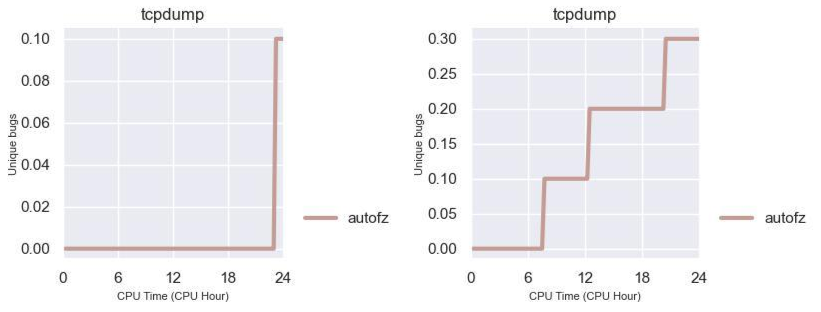
\includegraphics[width=0.52\textwidth]{figs/tcpdump_compare_orig_arm64_ub.png}
    \centering
    \caption{A comparison of bug discovery in AMD64 \texttt{autofz} and our ARM64 implementation
    coverage during fuzzing of tcpdump}
    \label{figs:tcp_compare_orig_arm64_ub.png}
\end{figure}

In addition to producing an ARM64 compatible \texttt{autofz}, we identified a potential improvement for \texttt{autofz}.
Existing versions of \texttt{autofz} use bitmap coverage to rank fuzzers during the preparation, but bitmap
coverage may not be the best metric for identifying the most effective fuzzers for a target. While
bitmap coverage indicates the portion of a target that was fuzzed, it does not guarantee bug discovery.
To resolve these problems, we plan to modify \texttt{autofz}, so fuzzers that discover more bugs during the
preparation phase are rewarded with more resources during the focus phase because discovering more bugs
across a smaller area of code decreases the attack surface by more entry points than discovering fewer
bugs over a greater area of the code.